\documentclass[11pt]{article}
\newcommand\Decide[1]{#1}
\makeatletter
\def\sectionsuffix      {}
\def\subsectionsuffix   {\quad}
\def\subsubsectionsuffix{\quad}
\def\paragraphsuffix    {\quad}
\renewcommand\@seccntformat[1]{\csname the#1\endcsname\csname#1suffix\endcsname}
\renewcommand\thesection{\protect\Decide{\@arabic\c@section}}
\renewcommand\thesubsection{\@arabic\c@section.\@arabic\c@subsection}
\makeatother

\usepackage{tabularx}
\usepackage{hyphenat}
\usepackage[utf8]{inputenc}
\usepackage{lmodern,textcomp}
\usepackage{enumitem}
\usepackage{ltablex}
\usepackage[english]{babel}
\usepackage{blindtext}
\usepackage{microtype}
\usepackage{hanging}
\usepackage[paperheight=279.4mm,paperwidth=210mm,left=20mm,right=20mm,top=20mm,footskip=10mm]{geometry}
\usepackage[final]{pdfpages}
\usepackage{tocloft}
\usepackage{setspace}
\usepackage[bottom,flushmargin]{footmisc}
\usepackage[sfdefault, light]{roboto}
\usepackage{graphicx}
\usepackage{subcaption}

\setlength\cftparskip{5pt}
\setlength\cftbeforesecskip{5pt}
\setlength\cftaftertoctitleskip{10pt}

\usepackage{fancyhdr}
\setlength{\parskip}{1em}
\setlength\parindent{0pt}

\setlist[itemize]{leftmargin=*}


\usepackage{titlesec}

\titlespacing\chapter{0pt}{12pt}{-5pt}
\titlespacing\section{0pt}{12pt plus 4pt minus 2pt}{-5pt plus 2pt minus 2pt}
\titlespacing\subsection{0pt}{12pt plus 4pt minus 2pt}{-5pt plus 2pt minus 2pt}
\titlespacing\subsubsection{0pt}{12pt plus 4pt minus 2pt}{-5pt plus 2pt minus 2pt}


\usepackage{titling}

\setlength{\droptitle}{-6em}
\usepackage{hyperref}
\hypersetup{
	colorlinks=true,
    linkcolor=[RGB]{56, 97, 246},
    pdfpagemode=FullScreen,
    unicode=false,
    pdftoolbar=true,
    pdfmenubar=true,
    pdffitwindow=false,
		pdfstartview={FitH},
    pdftitle={Teaching Portfolio - Anthony Kevins},
    pdfauthor={Anthony Kevins},
    pdfsubject={Teaching Portfolio},
    bookmarksopen=true,
    bookmarksopenlevel=2,
    pdfstartview=Fit,
    pdfpagemode=UseOutlines,
	pdfnewwindow=true,
	pdfborder={0 0 0}
}
\usepackage{bookmark}

\begin{document}
\begin{spacing}{0}
	\title{\huge \textbf{Teaching Portfolio}}
	\author{\LARGE Anthony Kevins}
	\date{Senior Lecturer in Politics and International Studies \endgraf
	Department of International Relations, Politics, and History \endgraf 
	Loughborough University}
	
	\maketitle
	
\end{spacing}

\tableofcontents

\bigskip
\setlength\fboxsep{0.25cm}
\noindent\fbox{%
	\parbox{\textwidth}{%
		\textbf{Summary of Qualifications}: 
		\begin{itemize}[itemsep=0em]
			\item Fellow of the Higher Education Academy	
			\item Teaching experience on undergraduate and graduate courses, covering a range of topics in Comparative Politics, Political Behaviour, IR, Political Theory, and Research Methods
			\item Extensive pedagogical training, including via a 5-ECTS Pedagogical Programme for Assistant  \mbox{Professors} at Aarhus University and the New Lecturers Programme at Loughborough University
		\end{itemize}
	}%
}


\newpage

\section{ Teaching Philosophy, Strategies, and Goals}

My teaching is shaped by the belief that an accessible political science education has the potential to help form not only good political scientists, but also good citizens. In an age in which formulaic talking points often pass for quality political discourse, I believe that political science can help students move beyond facile arguments by improving their substantive political knowledge, scientific literacy, and critical reasoning skills. As a teacher, my task is to facilitate this growth by encouraging students to actively engage with both the course material and their peers. I do so by employing pedagogical best-practices tied to constructive alignment, active learning, and an open dialogue with students.

My course development centres around the notion that intended learning outcomes, active learning activities, and student assessment tasks should all be closely aligned (i.e. constructive alignment). The first step in this process is the careful defining of learning objectives. Outlining these goals helps to maintain consistency across the course materials and assessment methods, while also ensuring that students are familiar with the skills they are meant to develop. For example, in \textit{Political Institutions}, an undergraduate core course that I co-developed and co-taught, the compendium (see \hyperref[sec:compendium]{Section 4.1}) laid out the learning objectives for the course as a whole and for each of the individual weeks. By specifying in advance not only every lecture's theoretical and empirical objectives, but also the corresponding tutorial's theory-application objectives, we were able to ensure a clear thread throughout the semester. 

Having identified learning goals, I then develop individual lesson plans that allow me to build toward the intended learning outcomes in an engaging way. In a master's-level seminar course on \textit{Democracy and Representation} (see \hyperref[sec:syllabus]{Section 4.2}), for example, I opened each class with a brief discussion of a contemporary political issue connected to the lesson's topic. Two goals guided this introductory framing: first, to tie the readings to current events and controversies, thereby highlighting the practical relevance of the course material; and second, to set the stage for theory-application later in the lesson, ensuring students have weekly opportunities to apply theories from the curriculum to real-world cases. 

Because this higher-level engagement requires a strong grasp of the assigned material, my lesson planning is also attuned to assuring student understanding and trying to mitigate against any ``hidden curriculum'' effects. After connecting the week's topic to contemporary events or debates, I lay out a road map for the class by providing a set of questions they should be able to answer by the end of the day's session. I revisit key concepts over the course of the lesson through a combination of lecturing and active learning activities, having students, typically in pairs or small groups, engage with questions of understanding. These latter activities have taken a variety of formats, including Vevox quizzes (followed by peer and then class-wide discussions), flipped classroom activities where students do the teaching, and reflections on the ``muddiest'' point of the lesson. (See \hyperref[sec:activities]{Section 4.3} for examples of how I do this in a lecture setting.) These techniques allow me to ascertain how well students have grasped the course material while at the same time encouraging peer-to-peer explanation -- which, in turn, helps to facilitate active learning and address variation in student backgrounds.

Once students have a reasonable grasp of the material, I move on to more advanced learning objectives. While these goals vary based on the level and subject of a given course, this deeper exploration of a topic often involves several steps: applying an argument or theory to an event or case; analysing the case from an alternative framework; and using the Socratic method to have students reflect upon any underlying assumptions. Furthermore, in-class discussions and debates are complemented by a variety of pre-class activities, including the preparation of small written assignments, group presentations, or methods exercises (with the aid of original screencasts for more technical tasks). (See \hyperref[sec:tutorials]{Section 4.4} for examples.) These exercises help students to cement comprehension and refine the research, presentation, and writing skills that they will need after graduation.
    
My course design also incorporates various larger learning activities that punctuate the semester, with the aim of consolidating the skills and knowledge developed in individual lessons. In addition to standard class room activities and graded assessments (such as policy briefs, exams, and essays), my courses incorporate stats labs (including training on the use of Generative AI as a data analysis tool), review sessions, and writing workshops (see \hyperref[sec:workshop]{Section 4.5} for an example). Some of these activities clearly necessitate more teacher intervention than others, but I always ensure that peer feedback plays a central role. In having students assist and assess one another, I seek to: (1) equip them with tools to more critically evaluate their own work; and (2) help them to develop skills that align with the course's learning objectives and the associated assessment tasks. At the same time, this approach also generates more frequent feedback for students and a more participatory classroom dynamic.
    
The final defining feature of my pedagogical approach is an open dialogue with students. Achieving this dialogue involves expressly making the case for the teaching activities I employ and then offering students the chance to provide informal, anonymous feedback after the first month of the semester. In my experience, this back-and-forth typically engenders a greater openness to new activities on their part. For example, some students have initially expressed doubt that peer feedback could be useful, based on the belief that only comments from their eventual grader are important; yet I have found that if I explain the motivations for this approach in advance, they quickly come to recognize and appreciate its benefits. The corollary of this, however, is that I must demonstrate an honest openness to adapting my teaching and learning activities when students are left unconvinced or have suggestions for improvements. 

Overall, my teaching practices are grounded in two beliefs: that a strong, accessible political science education can provide tools to make us better citizens; and that advances in pedagogical research can help us to more effectively reach our teaching goals. I look forward to a career in which I continually improve my ability to teach and engage students, building from their feedback while experimenting with new pedagogical techniques. 

\section{ Teaching Experience}

My teaching experience includes undergraduate and graduate course development and instruction, in formats ranging from small seminars to large lectures involving hundreds of students. 

I have taught both methodological and substantive subject matter, covering topics in Comparative Politics, Political Behaviour, IR, Political Theory, and Research Methods. I have also supervised dozens of undergraduate dissertations, assisted with students' research designs, and delivered quantitative methods training for their projects. 

In what follows, I briefly lay out an overview of some of my teaching. The syllabi for two of these courses (marked with asterisks) are subsequently provided in \hyperref[sec:materials]{Section 4}, which also includes a sample of other materials that I have used in my teaching. Please note, however, that as Loughborough University owns the copyright to my current teaching materials, they have not been included in the sample appendix content -- though I am of course happy to discuss my more recent teaching further if you get in touch. 

\subsection{Current Teaching}
\textbf{Capitalism, Democracy and the State}
	      \begin{itemize}[itemsep=0em, topsep=0em, partopsep=0em]
	      	\kern-\parskip\item Overview: Bachelor’s Course, Loughborough University (Standard Enrolment: $\sim$ 90).
	      	\item Duties Performed: Module leader, course design, lectures, seminars, coursework/exam design, and grading.
	      	\item Course Description: An introduction to Comparative Political Economy divided into three sections: institutions, politics, and public opinion. 
	      	\item Sample Topics: Varieties of Capitalism; Interest-Based Politics; Social Policy Preferences.
	      \end{itemize}
	\textbf{Introduction to Philosophy}
	      \begin{itemize}[itemsep=0em, topsep=0em, partopsep=0em]
	      	\kern-\parskip\item Overview: Bachelor’s Core Course (PPE Programme), Loughborough University (Standard Enrolment: $\sim$ 50).
	      	\item Duties Performed: Module leader, three lectures, three seminars, coursework design, and grading.
	      	\item Course Description: An introductory course designed to provide PPE students with an overview of central debates, figures, and topics in philosophy. 
	      	\item Sample Topics: Justice; Liberty; Equality.
	      \end{itemize}
		  \textbf{Politics and Government}
	      \begin{itemize}[itemsep=0em, topsep=0em, partopsep=0em]
	      	\kern-\parskip\item Overview: Bachelor’s Core Course, Loughborough University (Standard Enrolment: $\sim$ 200).
	      	\item Duties Performed: Module leader, course design, lectures, exam design.
	      	\item Course Description: A survey course providing an introduction to comparative politics alongside core data literacy training. 
	      	\item Sample Topics: Electoral Systems; Party Systems; Assessing Data Quality; Interpreting Data.
	      \end{itemize}

	\subsection{Past Teaching}
		  \textbf{British Politics and Government}
	      \begin{itemize}[itemsep=0em, topsep=0em, partopsep=0em]
	      	\kern-\parskip\item Overview: Bachelor’s Core Course, Loughborough University (Standard Enrolment: $\sim$ 200).
	      	\item Duties Performed: Course design, lectures, seminars, exam design, and grading.
	      	\item Course Description: A survey course providing an overview of British Politics and introducing students to the study of comparative politics. 
	      	\item Sample Topics: Comparative Methods; Constitutional Review; The Prime Minister and Cabinet.
	      \end{itemize}
	\textbf{Comparative European Politics}
	      \begin{itemize}[itemsep=0em, topsep=0em, partopsep=0em]
	      	\kern-\parskip\item Overview: Bachelor’s Course, Loughborough University (Standard Enrolment: $\sim$ 90).
	      	\item Duties Performed: Weekly seminars and grading.
	      	\item In-Class Teaching Time: Approximately 44 hours. 
	      	\item Course Description: A survey course combining an overview of comparative institutions and contemporary issues in European politics.
	      	\item Sample Topics: Governments and Parliaments; Politics, Markets, \& the Welfare State; The Politics of Globalisation and Immigration.
	      \end{itemize}
	\textbf{Political Institutions}*
	      \begin{itemize}[itemsep=0em, topsep=0em, partopsep=0em]
	      	\kern-\parskip\item Overview: Bachelor’s Core Course, Aarhus University (Standard Enrolment: $\sim$ 315).
	      	\item Duties Performed: Course design, lectures, exam design, and weekly seminars.
	      	\item Course Description: A survey course on institutionalism and various domestic and supranational institutions, with a particular focus on the EU.
	      	\item Sample Topics: Electoral Systems and Party Systems; Federalism; Executive Politics in the EU.
	      \end{itemize}
		  \textbf{Politics: Contemporary Europe}
	      \begin{itemize}[itemsep=0em, topsep=0em, partopsep=0em]
	      	\kern-\parskip\item Overview: Bachelor’s Course, McGill University (Standard Enrolment: $\sim$ 50).
	      	\item Duties Performed: Course design, lectures, exam design, and grading.
	      	\item Course Description: A survey of welfare state, capitalist, and citizenship regime typologies, as well as the policy changes across them.
	      	\item Sample Topics: Towards a Two-Tiered Welfare State?; Is European Capitalism Different?; How do Different Types of Nationalism Affect Tolerance? 
	      \end{itemize}
		  \textbf{Smart Scholarship}
	\begin{itemize}[itemsep=0em, topsep=0em, partopsep=0em]
		\kern-\parskip\item Overview: Bachelor’s Core Course, Loughborough University (Standard Enrolment: $\sim$ 20).
		\item Duties Performed: Weekly seminars and grading.
		\item Course Description: A skills course for incoming BA students, covering topics such as critical analysis, effective communication, and original research.
		\item Sample Topics: Analysing a Text; Understanding Frameworks and Theories; Showcasing Presentations.
	\end{itemize}
	\textbf{Democracy and Representation}*
	      \begin{itemize}[itemsep=0em, topsep=0em, partopsep=0em]
	      	\kern-\parskip\item Overview: Master’s Seminar, Aarhus University (Standard Enrolment: $\sim$ 10).
	      	\item Duties Performed: Course design, instruction, exam design, and grading.
	      	\item Course Description: An exploration of the bi-directional link between public opinion and policy making, including patterns of unequal representation.
	      	\item Sample Topics: The Survey Method; Uses and Abuses of Public Opinion Data; Democracy in the European Union.
	      \end{itemize}
	\textbf{Pragmatism and Politics}
	      \begin{itemize}[itemsep=0em, topsep=0em, partopsep=0em]
	      	\kern-\parskip\item Overview: Master’s Seminar, Aarhus University, Spring 2015 (Standard Enrolment: $\sim$ 5).
	      	\item Duties Performed: Course design, instruction, exam design, and grading.
	      	\item Course Description: An examination of the challenges underlying the balance between technocracy and democracy.
	      	\item Sample Topics: The End of Ideology; Philosophical versus Everyday Pragmatism; A Democratic Deficit?
	      \end{itemize}
		  \textbf{Social Science Methods for Journalists}
	      \begin{itemize}[itemsep=0em, topsep=0em, partopsep=0em]
	      	\kern-\parskip\item Overview: Master’s Core Course, Aarhus University (Standard Enrolment: $\sim$ 80).
	      	\item Duties Performed: Course design, lectures, exam design, grading, and weekly seminars.
	      	\item Course Description: An introduction to social science research design and methods (both quantitative and qualitative).
	      	\item Sample Topics: Case Selection and Data Sampling; Designing and Conducting Interviews and Surveys; Introduction to Statistical Inference.
	      \end{itemize}

\subsection{Other Teaching}
In addition to my university-level teaching, I have years of experience teaching in other settings. 

Prior to pursuing my PhD, I worked as a math teacher at a private high school in Toronto, where I taught grade 12 courses covering calculus, vector algebra, advanced functions, and finite mathematics. I also taught English to school children in Italy for a summer, and spent several years teaching preparatory courses for standardized tests (i.e., the SAT, GRE, and GMAT).

\section{ Professional Development}

I am a Fellow of the Higher Education Academy and have completed a host of pedagogical training, most notably via Loughborough University's New Lecturers Programme (2019-2022) and a (5-ECTS) Teacher Training Programme for Assistant Professors at Aarhus University (2016-2017). 
	 
I have also attended a wide array of additional pedagogical training sessions hosted by Loughborough University's Centre for Academic Practice and by Aarhus University's Centre for Teaching and Learning. These sessions covered topics such as inclusive teaching in multicultural contexts, PhD supervision techniques, and the use of active learning in large-class settings.
		
Finally, I have participated in a variety of technology-centred training (offered by Loughborough University's Centre for Academic Practice). This has included training on adapting to changing circumstances (e.g., Running Dual Delivery Teaching Sessions) and updating and refining my use of educational IT (e.g., Vevox for Advanced Users, Using MS Teams to Support Group Work). 

\section{ Sample Teaching Materials}
\label{sec:materials}

This section presents the compendium for the bachelor's core course that I co-developed and co-taught, as well as a syllabus from one of my graduate seminars. It then provides several examples of other teaching materials that I have employed: five in-lecture activities; two seminar group exercises; and a writing workshop activity.\\


\includepdf[pages=1,pagecommand={\thispagestyle{plain}\subsection{Undergraduate Course Compendium}\label{sec:compendium}},
height=\textheight,keepaspectratio,trim=80pt 80pt 80pt 80pt]{Undergraduate.pdf}

\includepdf[pages=2-21,pagecommand={},height=\textheight,keepaspectratio,trim=80pt 80pt 80pt 80pt]{Undergraduate.pdf}
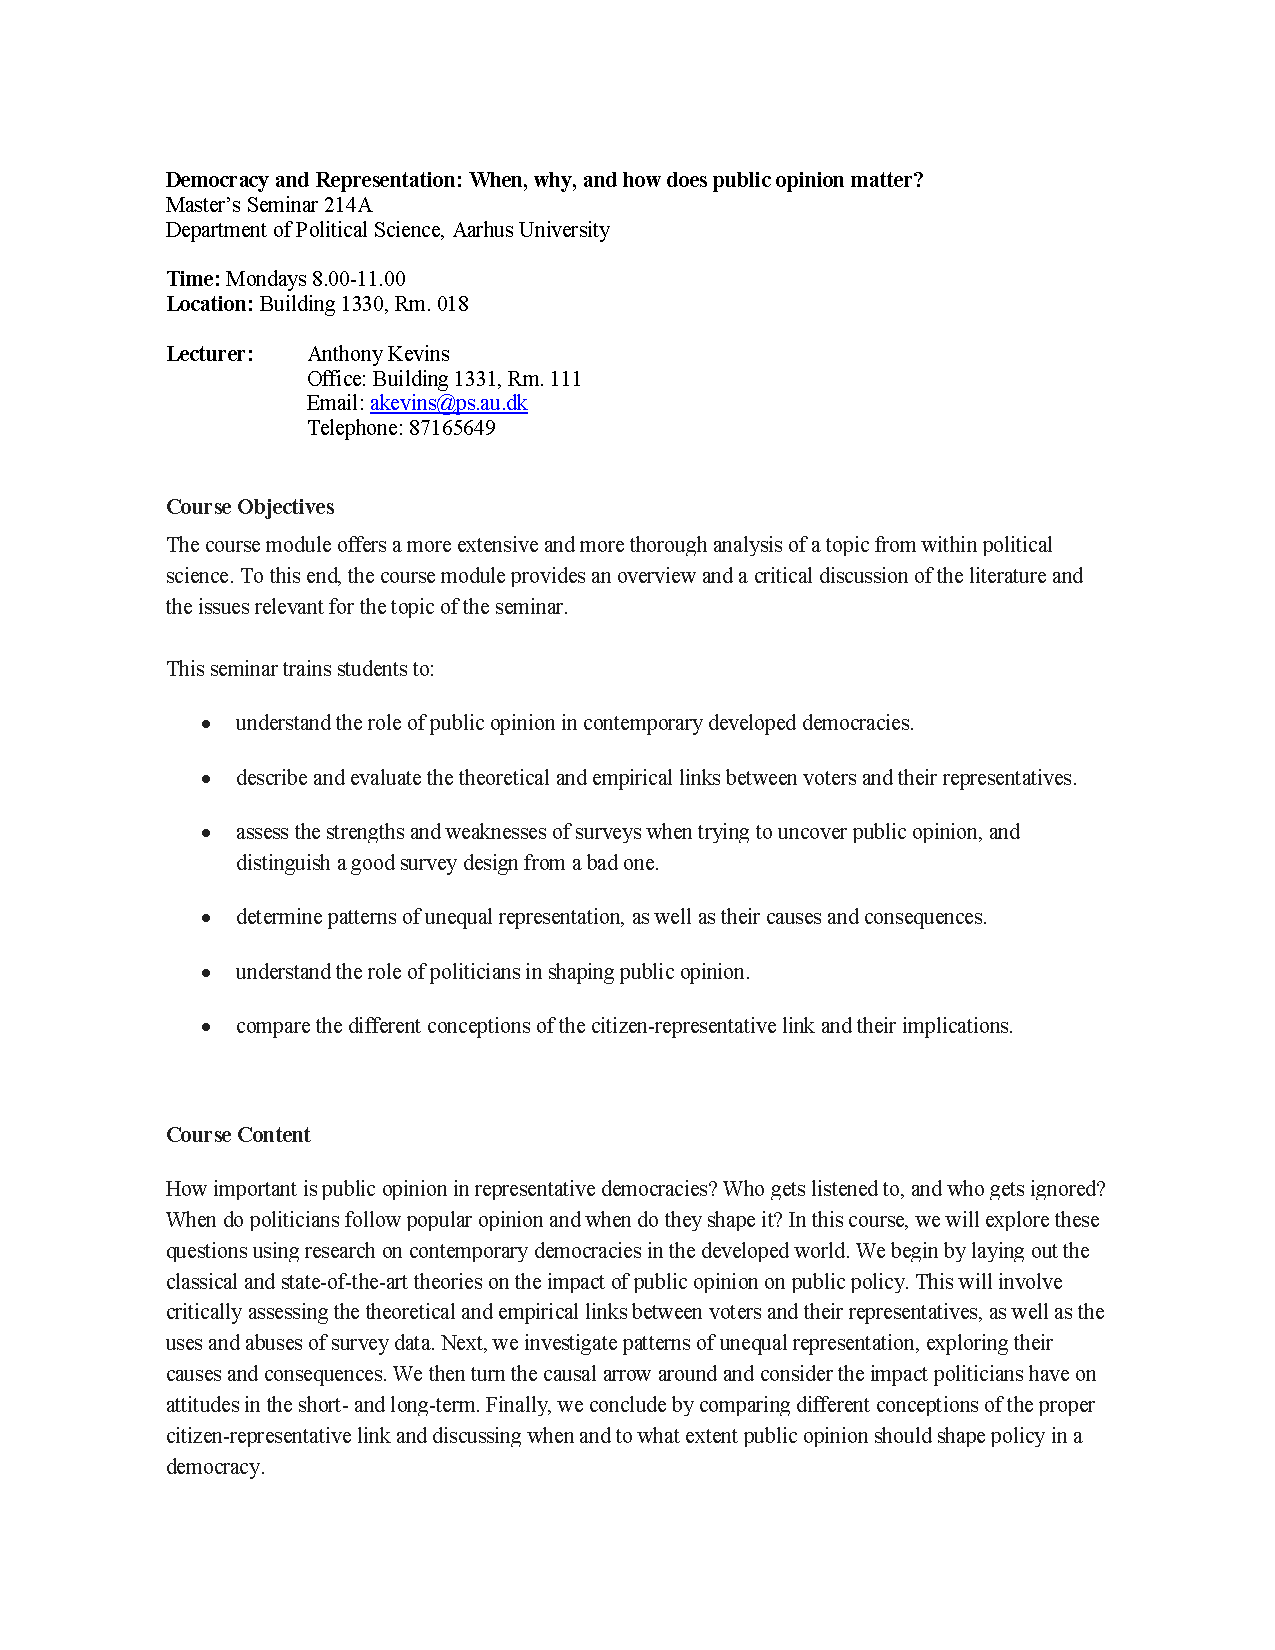
\includepdf[pages=1,pagecommand={\thispagestyle{plain}\subsection{Graduate Seminar Syllabus}\label{sec:syllabus}},height=\textheight,keepaspectratio,trim=60pt 60pt 60pt 60pt]{Graduate.pdf}
\includepdf[pages=2-7,pagecommand={},height=\textheight,keepaspectratio,trim=60pt 60pt 60pt 60pt]{Graduate.pdf}
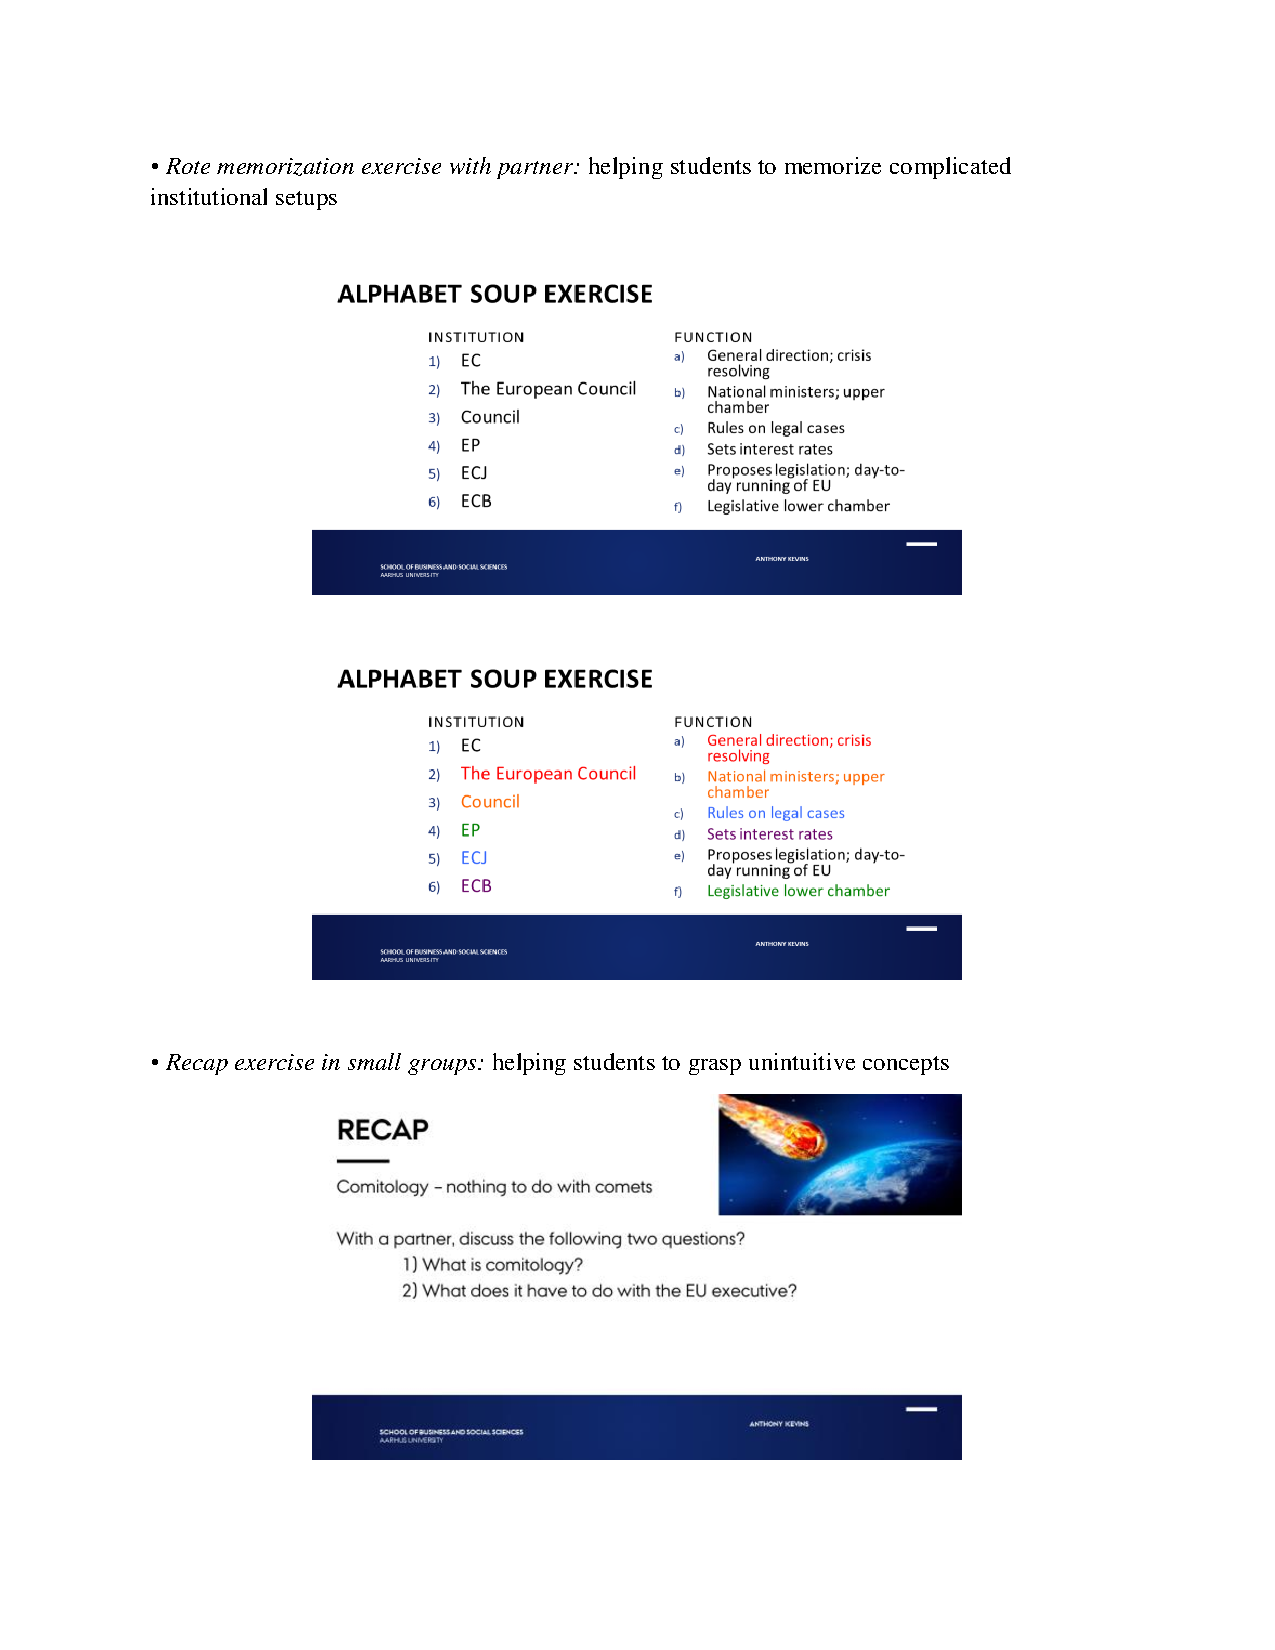
\includepdf[pages=1,pagecommand={\thispagestyle{plain}\subsection{Lecture Activities}\label{sec:activities}},height=\textheight,keepaspectratio,trim=60pt 60pt 60pt 60pt]{Lectures.pdf}
\includepdf[pages=2-3,pagecommand={},height=\textheight,keepaspectratio,trim=60pt 60pt 60pt 60pt]{Lectures.pdf}
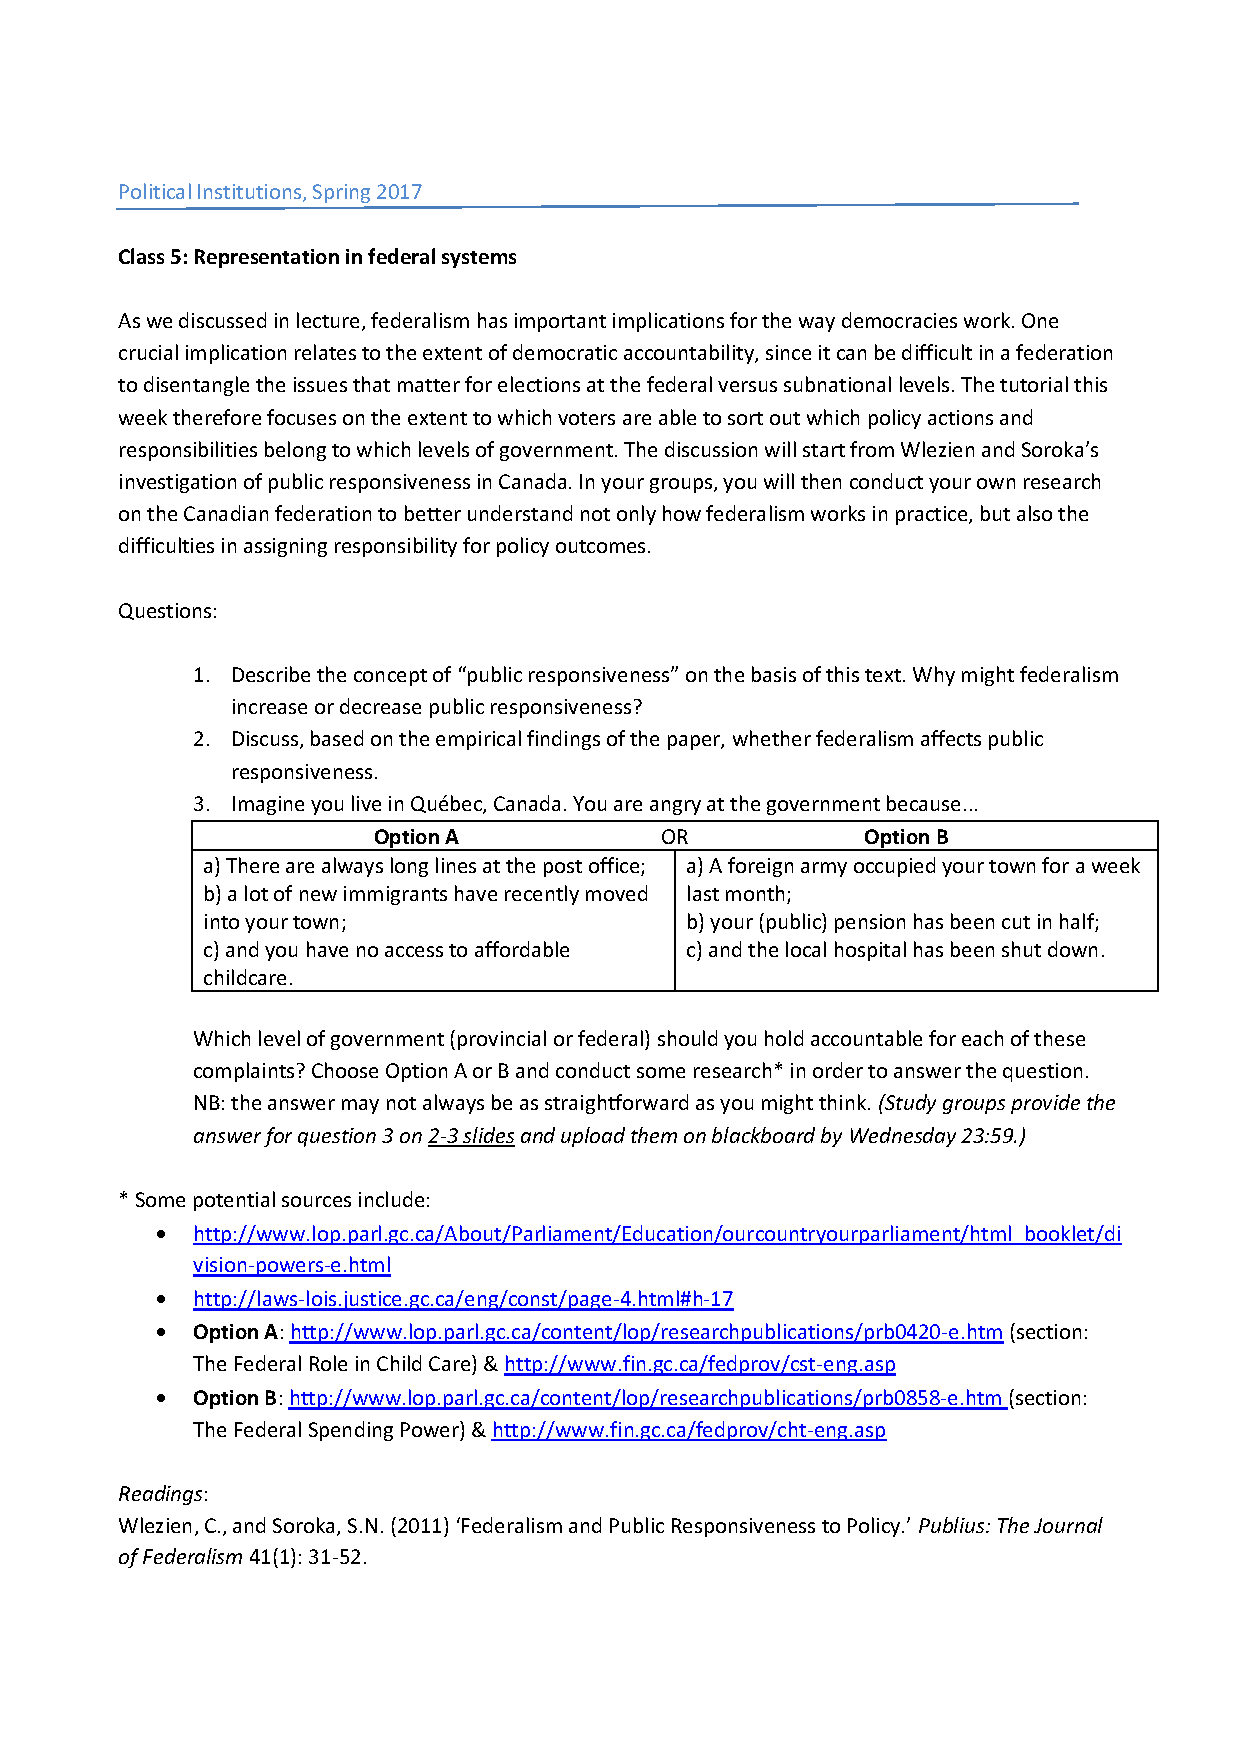
\includepdf[pages=1,pagecommand={\thispagestyle{plain}\subsection{Group Exercises}\label{sec:tutorials}},height=\textheight,keepaspectratio,trim=60pt 60pt 60pt 60pt]{Tutorial1.pdf}
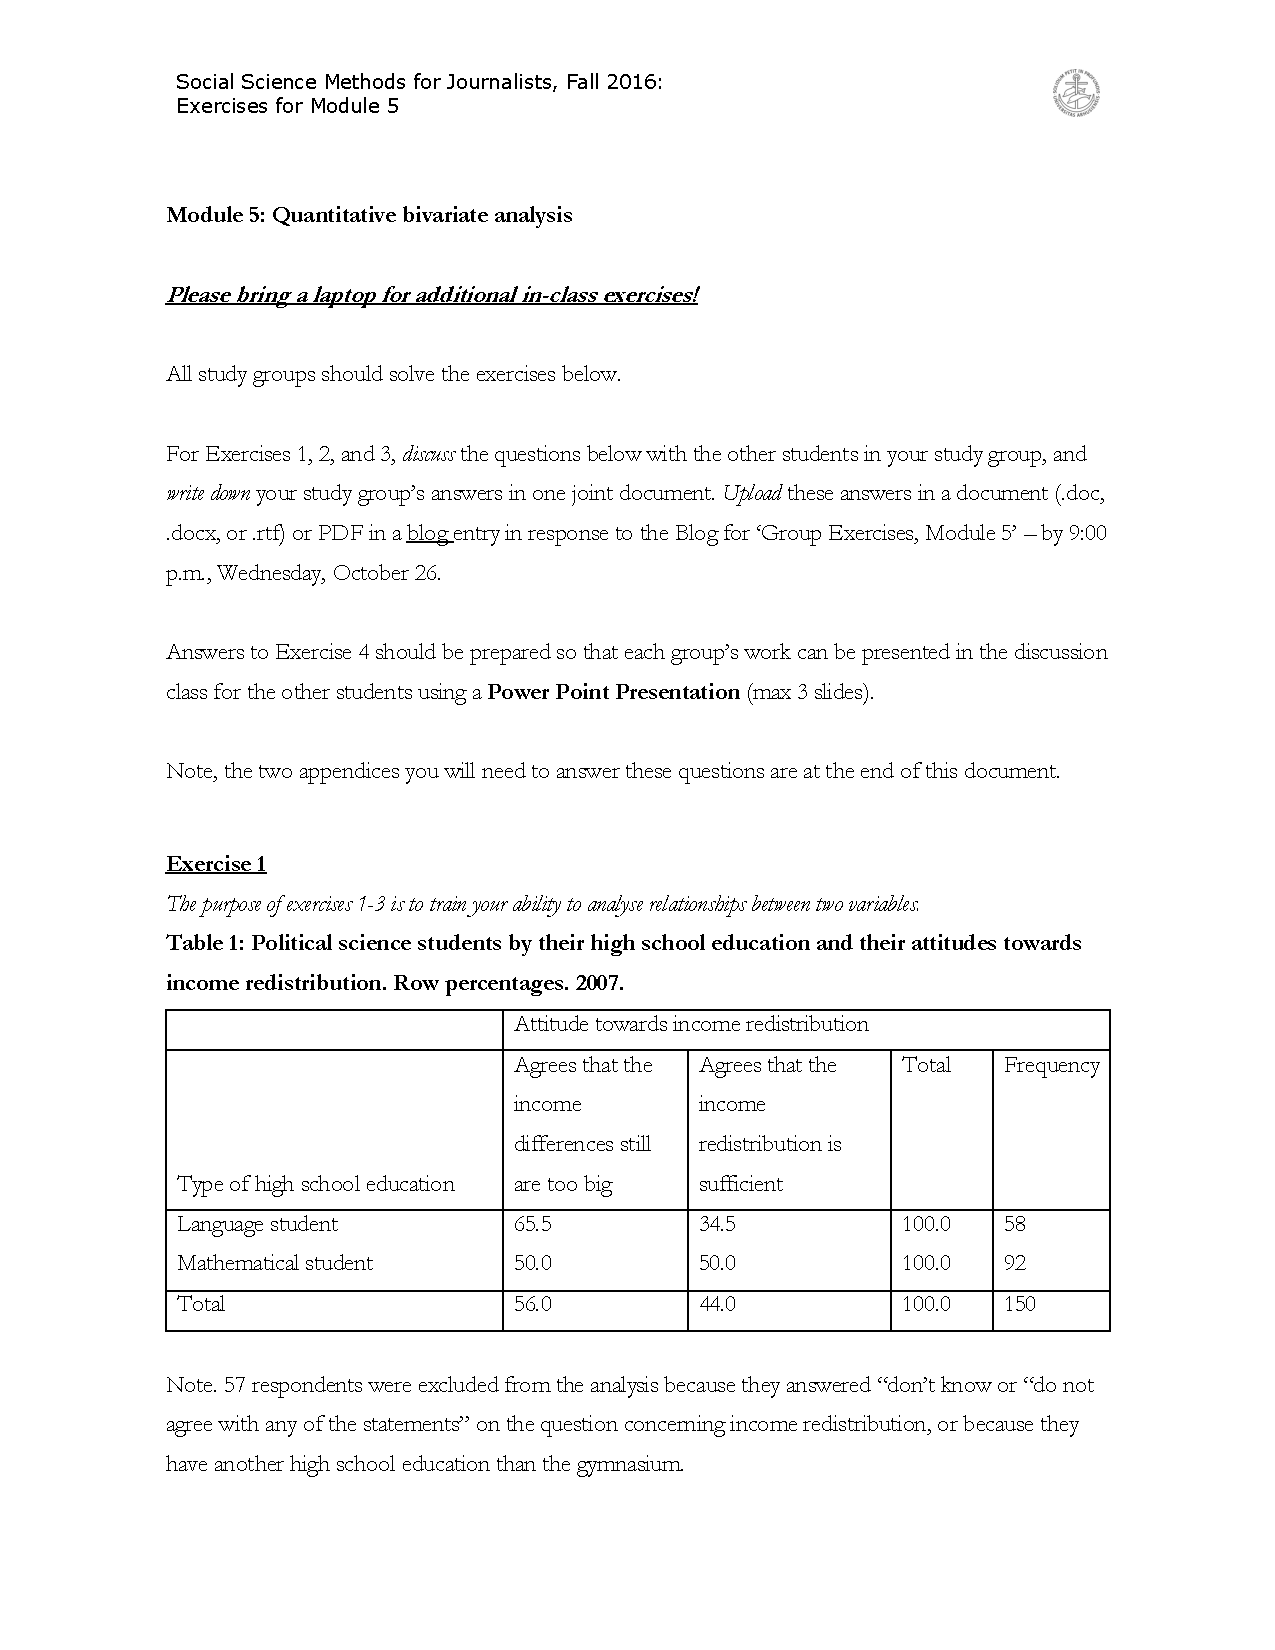
\includepdf[pages=-,pagecommand={},height=\textheight,keepaspectratio,trim=60pt 60pt 60pt 60pt]{Tutorial2.pdf}
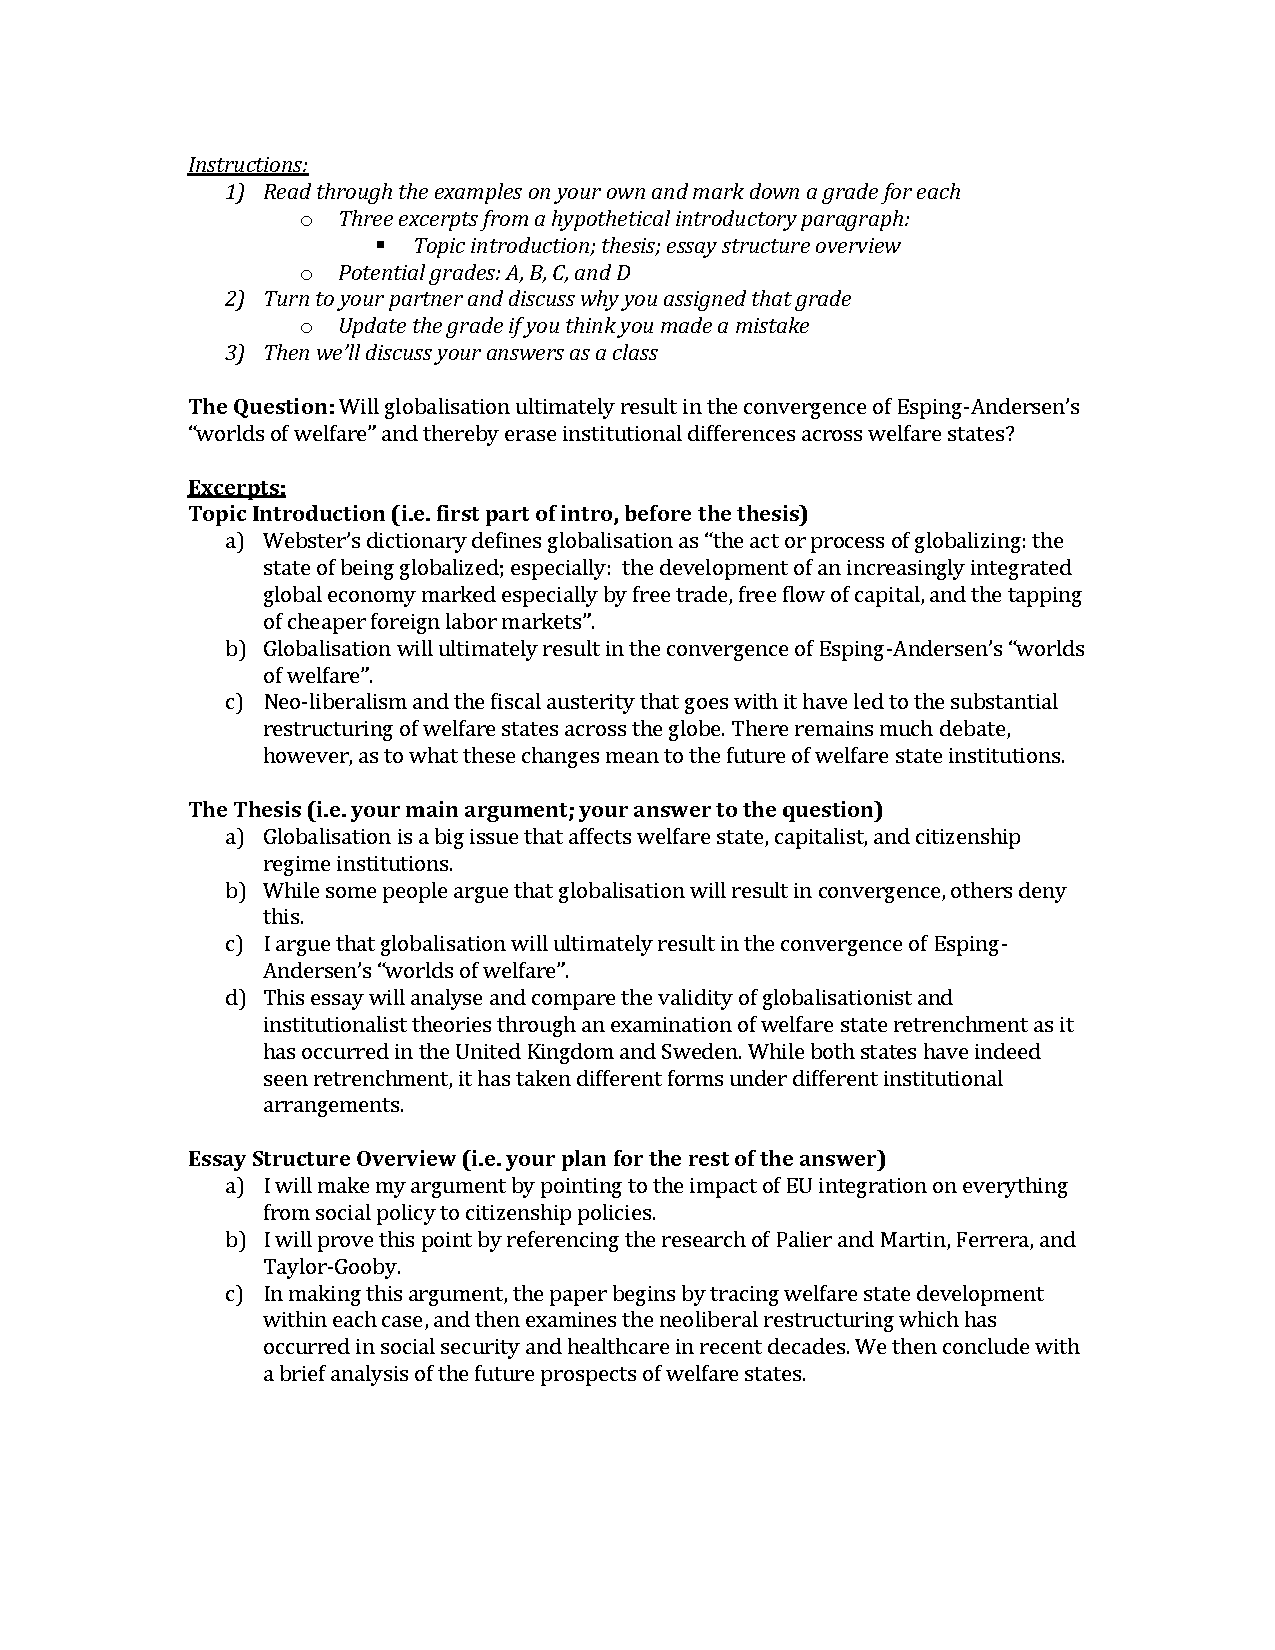
\includepdf[pages=1,pagecommand={\thispagestyle{plain}\subsection{Writing Workshop Activity}\label{sec:workshop}},height=\textheight,keepaspectratio,trim=60pt 60pt 60pt 60pt]{Workshop.pdf}


\section{ Evaluations of Teaching}

The remainder of the teaching portfolio contains evaluations of my teaching. This section begins with feedback from Ole Lauridsen, who is the Deputy Director of Aarhus University’s Centre for Teaching and Learning. I received the attached letter as formal feedback after he sat in on one of my classes as part of a pedagogical course. The rest of the section then provides a varied selection of student evaluations from my courses, which are presented here in chronological order. (Please note that a few of the student comments are written in Danish.)


\includepdf[pages=36,pagecommand={\thispagestyle{plain}\subsection{Teaching Supervision Feedback}},height=\textheight,keepaspectratio,trim=50pt 50pt 50pt 50pt]{Appendix_Materials.pdf}

\includepdf[pages=37,pagecommand={\thispagestyle{plain}\subsection{Student Evaluations}},width=\textwidth,height=\textheight,keepaspectratio,trim=30pt 30pt 30pt 30pt]{Appendix_Materials.pdf}
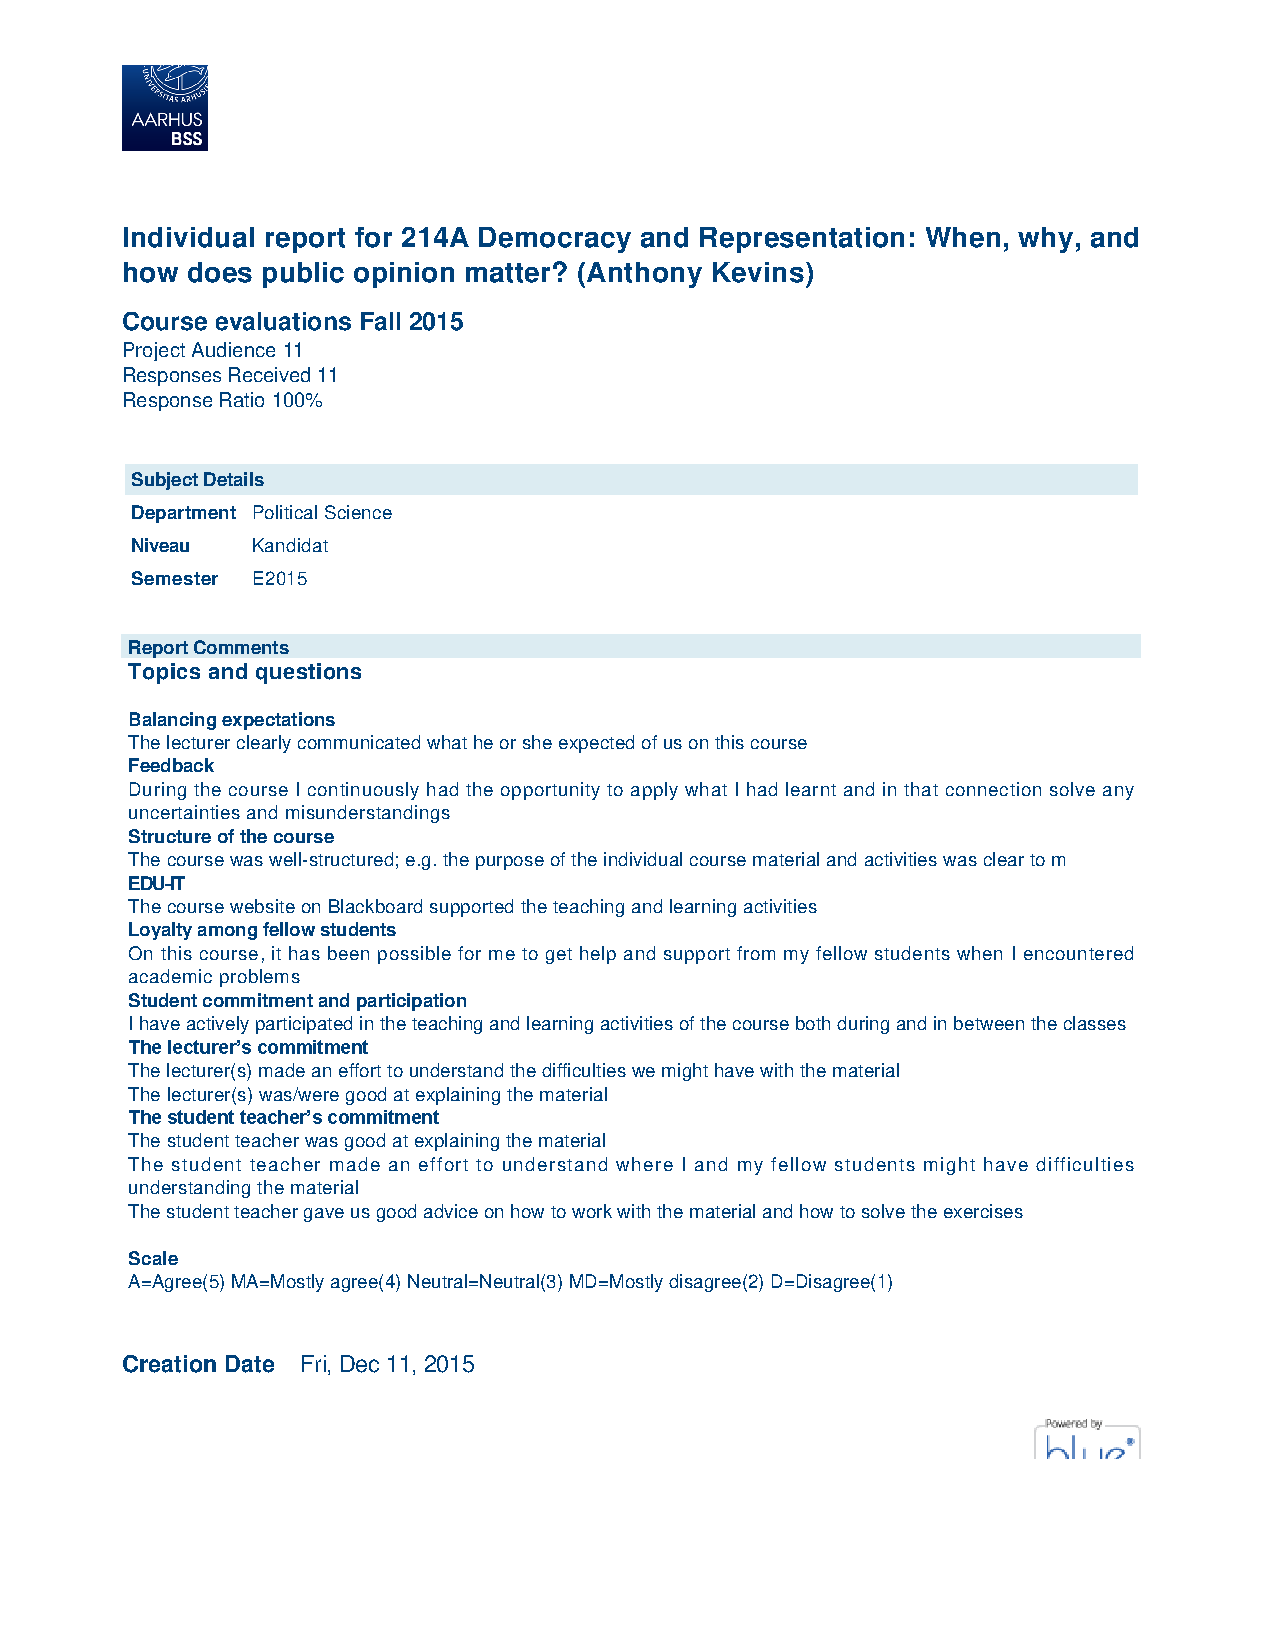
\includepdf[pages=-,pagecommand={},width=\textwidth,height=\textheight,keepaspectratio,trim=30pt 30pt 30pt 30pt]{Evaluations2.pdf}

\begin{figure}
	Political Institutions, Aarhus University\par\medskip
	\centering
	\begin{subfigure}{\textwidth}
		\includegraphics[page=68,viewport=0 396 612 800,width=\textwidth,clip]%
		{Appendix_Materials.pdf}
	\end{subfigure}\\
	\begin{subfigure}{\textwidth}
		\includegraphics[page=69,viewport=0 396 612 800,width=\textwidth,clip]%
		{Appendix_Materials.pdf}
	\end{subfigure}\\
\end{figure}

\begin{figure}
	Political Institutions, Aarhus University\par\medskip
	\centering
	\begin{subfigure}{\textwidth}
		\includegraphics[page=72,viewport=0 396 612 800,width=\textwidth,clip]%
		{Appendix_Materials.pdf}
	\end{subfigure}\\
	\begin{subfigure}{\textwidth}
		\includegraphics[page=73,viewport=0 396 612 800,width=\textwidth,clip]%
		{Appendix_Materials.pdf}
	\end{subfigure}\\
\end{figure}

\end{document}